\section{Basics}

알고리즘은 문제 해결을 위한 일련의 구체적인 동작. 자연어, 의사 코드, 플로우 차트 등으로 표현 가능. 시간복잡도는 알고리즘의 기본적인 연산(대입, 비교, 산술 등) 횟수를 입력 크기에 대한 함수로 나타낸다. 이렇게 표현하기 위해 점근적 표기를 사용한다.

\begin{figure}[h]
  \centering
  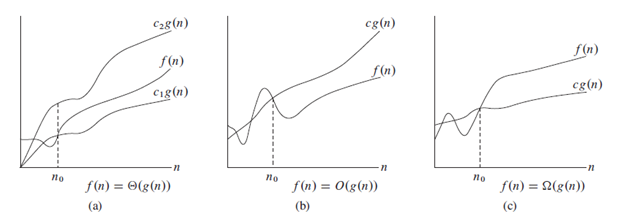
\includegraphics[width=\columnwidth]{asymptotic-notation-graphs.png}
\end{figure}

\begin{enumerate}[(a)]
  \item $\Theta$: $n_0$ 보다 큰 모든 $n$에 대해 상한과 하한을 동시에 만족. 즉, $O$과 $\Omega$가 동일한 경우. average case.
  \item $O$: $n$이 증가함에 따라 $O(g(n))$이 점근적 상한. 즉, $g(n)$은 $f(n)$의 상한. $g(n)$이 $n_0$보다 큰 모든 $n$에 대해 항상 $f(n)$보다 크다. worst case.
  \item $\Omega$: $n$이 증가함에 따라 $\Omega(g(n))$이 점근적 하한. 즉, $g(n)$은 $f(n)$의 하한. $g(n)$이 $n_0$보다 큰 모든 $n$에 대해 항상 $f(n)$보다 작다. best case.
\end{enumerate}

보통 시간복잡도를 $O$ 표기로 나타내는데, 실제로는 $\Theta$인 의미가 많음. 혹시 더 나은 방법이 있을지 모르기 때문에 $\Theta$ 표기를 지양함.

\begin{figure}[h]
  \centering
  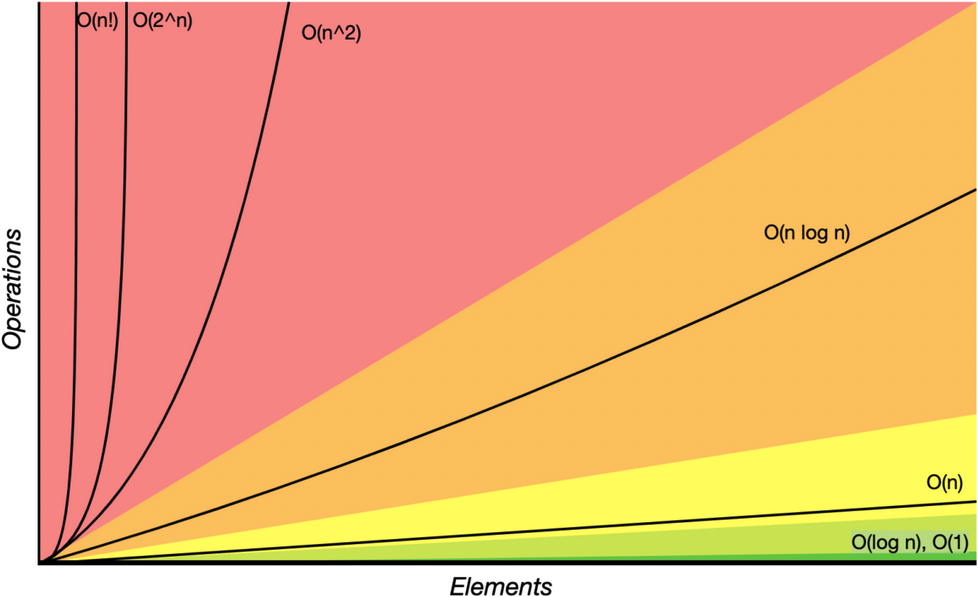
\includegraphics[width=\columnwidth]{big-o-complexity-chart.png}
\end{figure}

상각 분석은 점근적 분석과 달리 실제로 연산을 수행하여 총 연산 횟수의 합을 시행 횟수로 나누는 분석법.

\section{Divide and Conquer}

주어진 문제의 입력을 분할하여 문제를 해결하는 방식의 알고리즘. 문제의 크기가 매우 작으면 풀기 쉬워지는 경우, 또는 문제의 크기를 줄이면 trivial solution에 가까워지는 경우 사용한다.

입력 크기가 $n$일 때 1회 분할마다 각각의 입력 크기가 반감하기 때문에, $k$회 분할하는 경우 각각의 입력 크기는 $n / 2^k$이며, 입력 크기가 1이 되면 더 이상 분할 할 수 없으므로 $k = \log_2{n}$이다.

\begin{enumerate}[i.]
  \item 1회 분할했을 때 입력 크기: $n / 2$
  \item 2회 분할했을 때 입력 크기: $n / 2^2$
  \item k회 분할했을 때 입력 크기: $n / 2^k$
\end{enumerate}

분할로 인해 부분 문제가 매우 커지는 경우에는 부적절하다. 부분 문제의 취합 방법에 따라 분할 정복 알고리즘의 성능이 좌우된다.

\subsection{Merge Sort}

입력된 리스트를 두 부분으로 분할하여 각 부분 문제의 요소가 1개가 될 때까지 분할을 반복하고, 각 부분 문제를 정렬하며 병합하는 정렬 알고리즘.

\begin{verbatim}
def merge_sort(s: list[int]) -> list[int]:
  if len(s) <= 1: return s

  m = len(s) // 2
  l = merge_sort(s[:m])
  r = merge_sort(s[m:])

  li = ri = 0
  t = []
  while li < len(l) and ri < len(r):
    if l[li] < r[ri]:
      t.append(l[li])
      li += 1
    else:
      t.append(r[ri])
      ri += 1

  return t + l[li:] + r[ri:]
\end{verbatim}

분할 시 부분 문제가 $n / 2^k$개로 쪼개지므로 $O(\log{n})$이고, 각 층을 병합하는 데 $O(n)$ 시간이 걸리므로, 총 시간복잡도는 $O(n \log{n})$이다.

\subsection{Quick Sort}

머지 소트는 각 층에서 매번 새로운 리스트를 만들기 때문에 공간복잡도가 $O(n^2)$이다. 퀵 소트는 in-place 방식으로 구현할 수 있기 때문에 공간복잡도를 줄일 수 있다.

퀵 소트는 pivot을 기준으로 작은 수는 왼쪽으로, 큰 수는 오른쪽으로 분할하는 과정을 반복한다. 이를 partitioning이라고 한다.

\begin{verbatim}
def partition(a: list[int], si: int,
              ei: int, pi: int) -> int:
  pv = a[pi]
  a[si], a[pi] = a[pi], a[si]
  li, ri = si + 1, ei

  while li <= ri:
    while li <= ei and a[li] <= pv: li += 1
    while ri >= si and a[ri] > pv: ri -= 1
    if li <= ri:
      a[li], a[ri] = a[ri], a[li]
      li, ri = li + 1, ri - 1
  a[si], a[ri] = a[ri], a[si]

  return ri
\end{verbatim}

partitioning된 각 부분 문제에 대해 퀵 정렬을 재귀적으로 실행하면 된다.

\begin{verbatim}
def quick_sort(a: list[int], si: int,
               ei: int) -> None:
  if si >= ei: return

  rpi = random.randrange(si, ei)
  pi = partition(a, si, ei, rpi)

  quick_sort(a, si, pi - 1)
  quick_sort(a, pi + 1, ei)
\end{verbatim}

최악의 경우(항상 가장 작거나 큰 숫자가 pivot으로 선택되는 경우, 리스트가 이미 정렬되어 있는 경우) 시간복잡도는 $O(n^2)$이 된다. pivot을 랜덤하게 정했을 때 평균 시간복잡도는 $O(n \log{n})$. 성능 향상을 위해 부분 문제가 작아지면 삽입 정렬을 함께 사용하기도.

\subsection{Selection Problem}

$n$개의 숫자 중 $k$번째로 작은 숫자를 찾는 문제. 최소 숫자를 $k$번 찾으면 $O(kn)$, 리스트를 정렬하고 $k$번째 요소를 선택하면 $O(n \log{n})$ 시간이 걸린다. partition으로 이진 탐색을 하면 최악의 경우 $O(n \log{n})$.

pivot을 랜덤하게 정해 한쪽으로 치우치지 않는 최선의 경우로 분할하면 부분 문제 크기가 $(3/ 4)^in$배씩 줄어들기 때문에 최선의 경우 $O(\sum{(3 / 4)^in}) = O(n)$. 최선의 경우로 분할되는 확률은 $1 / 2$이므로 평균 시간복잡도는 $2 \times O(n) = O(n)$.

\begin{verbatim}
def selection(a: list[int], k: int,
              si: int, ei: int) -> int:
  if si >= ei: return

  rpi = random.randrange(si, ei)
  pi = partition(a, si, ei, rpi)
  ll = (pi - 1) - si + 1

  if ll >= k:
    return selection(a, k, si, pi - 1)
  elif k == ll + 1:
    return a[pi]
  rk = k - ll - 1
  return selection(a, rk, pi + 1, ei)
\end{verbatim}

\subsection{Closest Pair Problem}

2차원 평면 상에서 거리가 가장 가까운 한 쌍의 점을 찾는 문제. 모든 쌍의 조합을 계산한다면, ${}_{n}C_{2} = {n(n - 1) \over 2} = O(n^2)$. 대신 $n$개의 점을 $x$ 좌표 기준으로 오름차순 정렬하여 반으로 분할하고, 각각의 부분 문제에서 최근점 쌍을 찾으면 더 효율적.

이때 두 부분 사이에도 최근접 쌍이 존재할 수 있으므로 왼쪽 부분의 최근접 거리와 오른쪽 부분의 최근접 거리 중 더 작은 값을 $d$라고 하면, 왼쪽 부분의 맨 오른쪽 점의 $x$ 좌표에 $d$를 뺀 범위부터 오른쪽 부분의 맨 왼쪽 점의 $x$ 좌표에 $d$를 더한 범위까지에서도 최근접 쌍을 탐색해야 한다.

\subsection{Master Theorem}

분할 정복 알고리즘 분석법. $n$개의 문제를 분할 정복으로 해결할 때, $n$개의 문제를 $b$개의 부분 문제로 분할하고 이 중 $a$개의 부분 문제만 연산할 때 $f(n)$ 시간이 걸린다고 하면:
$$
T(n) = aT({n \over b}) + f(n)
$$

\subsubsection{Case 1}

문제를 분할, 정복하는 과정의 크기가 원 문제보다 작아지는 경우.
$$
\begin{aligned}
  &\text{When} \quad f(n) = O(n^c) \quad \text{where} \quad c < c_{crit} \\
  &\text{then} \quad T(n) = \Theta(n^{c_{crit}})
\end{aligned}
$$

이진 트리 전체 순회: $n$개의 문제를 2개($b = 2$)의 부분 문제로 나누고 이 중 2개($a = 2$)의 부분 문제애 대해 접근 연산($f(n) = O(1)$)한다.
$$
\therefore T(n) = 2T({n \over 2}) + O(1)
$$
이때 $O(n^c)$인데 $f(n) = O(1)$이므로, $c$는 0. 이어서 Case 1 문제인지 확인해본다. ($c < c_{crit}$)
$$
\begin{aligned}
  &\because c_{crit} = \log_b{a} = \log_2{2} = 1 > c \\
  &\therefore T(n) = \Theta(n)
\end{aligned}
$$

\subsubsection{Caes 2}

문제를 분할, 정복하는 과정의 크기가 원 문제와 비슷한 경우.
$$
\begin{aligned}
  \text{When} \quad f(n) &= \Theta(n^{c_{crit}} \log^k{n}) \\
  \text{then} \quad T(n) &=
  \begin{cases}
    \Theta(n^{c_{crit}} \log^{k + 1}{n}) &\text{if } k > -1 \\
    \Theta(n^{c_{crit}} \log \log{n}) &\text{if } k = -1 \\
    \Theta(n^{c_{crit}}) &\text{if } k > -1 \\
  \end{cases}
\end{aligned}
$$

머지 소트: $n$개의 문제를 2개($b = 2$)의 부분 문제로 나누고 이 중 2개($a = 2$)의 부분 문제에 대해 정렬 연산($f(n) = O(n)$)을 한다. 따라서,
$$
T(n) = 2T({n \over 2}) + O(n)
$$
이때 $f(n) = \Theta({n^c \log^k n})$인데 $f(n) = O(n)$이므로 $c = 1, k = 0$임을 알 수 있다. ($\because \log^0{n} = 1$) 이어서 Case 2a 문제인지 확인해본다. ($c = \log_b{a}$)
$$
\begin{aligned}
  \because c_{crit} &= \log_b{a} = \log_2{2} = 1 = c \\
  \therefore T(n) &= \Theta(n \log^{0 + 1}{n}) \\
  &= \Theta(n \log n)
\end{aligned}
$$

\subsubsection{Case 3}

문제가 오히려 커지는 경우.
$$
\begin{aligned}
  &\text{When} \quad f(n) = \Omega(n^c) \quad \text{where} \quad c < c_{crit} \\
  &\text{if} \quad af({n \over b}) <= kf(n) \quad \text{for} \quad k < 1 \\
  &\text{then} \quad T(n) = \Theta{f(n))}
\end{aligned}
$$

\section{Greedy}

최적화 문제를 해결하는 알고리즘. 항상 최적의 해를 찾는다는 의미가 아니라, 가능한 해들 중 가장 최적의 해를 찾는 것. 즉, 최적화에 '관한' 문제에 사용할 수 있다. 근시안적 선택으로 부분적인 최적해를 찾고, 이를 모아서 문제의 최적해를 찾는다. 한 번 선택한 데이터를 절대로 번복하지 않는 것이 특징.

\subsection{Minimum Spanning Tree (MST)}

가중치 그래프에서 사이클 없이 모든 점을 연결시킨 트리(spanning tree) 중 가중치 합이 최소가 되는 트리. spanning tree에는 항상 $n - 1$개의 간선이 있다. 그보다 많으면 반드시 사이클이 생긴다.

\subsubsection{Kruskal's Algorithm}

가중치 오름차순으로 $n$개 간선을 정렬하고, 순서대로(greedy하게) disjoint set에 추가하여 사이클을 방지한다. 이미 set에 간선이 있는 경우 스킵한다.

아래 구현한 disjoint set에서 \texttt{make}는 $O(1)$, \texttt{find}는 상각 분석으로 $\Theta(\alpha(n))$. 이때 $\alpha(n)$은 inverse ackemann funciton으로 매우 작은 값. \texttt{union}은 \texttt{find}와 동일한 시간복잡도.

\begin{verbatim}
class DisjointSet:
  def __init__(self) -> None:
    self.p: dict[str, str] = {}
    self.l: dict[str, int] = {}

  def make(self, x: str) -> None:
    self.p[x] = x
    self.l[x] = 1

  def find(self, x: str) -> str:
    r = x
    while self.p[r] != r:
      r = self.p[r]
    while self.p[x] != r:
      p = self.p[x]
      self.p[x] = r
    return r

  def union(self, x: str,
                  y: str) -> None:
    x = self.find(x)
    y = self.find(y)
    if x == y:
      return
    if self.l[x] < self.l[y]:
      x, y = y, x
    self.p[y] = x
    self.l[x] = self.l[x] + self.l[y]
\end{verbatim}

\texttt{union} 과정에서 최악의 경우 선형 트리가 만들어져 \texttt{find}에 $O(n)$ 시간이 소요될 수 있다.

\begin{figure}[h]
  \centering
  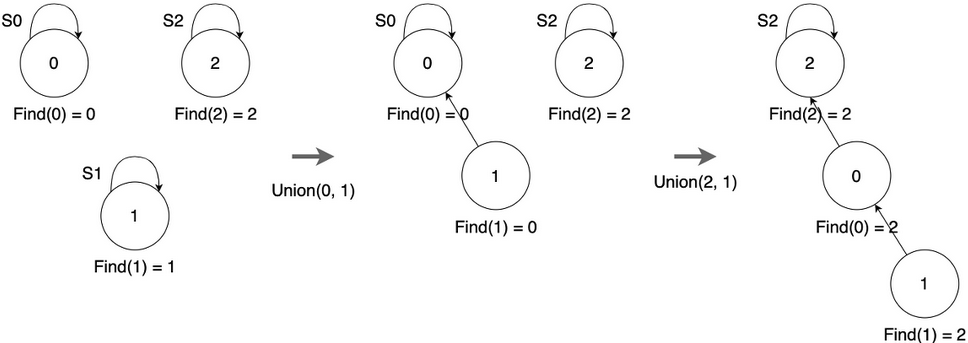
\includegraphics[width=\columnwidth]{disjoint-set-linear-tree.png}
\end{figure}

이를 방지하기 위해 \texttt{find}할 때마다 찾고자 한 $x$의 상위 노드가 루트 노드가 아닌 경우 $x$의 상위 노드를 루트로 갱신한다. 이렇게 하면 평평한 트리가 만들어져 차후 빠르게 \texttt{find}를 수행할 수 있음.

\begin{figure}[h]
  \centering
  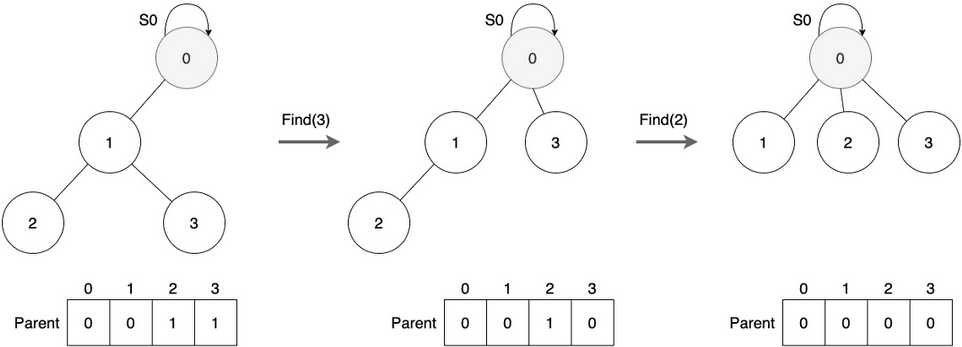
\includegraphics[width=\columnwidth]{disjoint-set-path-compression.png}
\end{figure}

kruskal's algorithm에서는 정렬에 가장 오랜 시간이 걸리므로 시간복잡도는 $O(n \log{n})$. 이때 $n$은 정점의 개수가 아닌 간선의 개수.

\begin{verbatim}
def kruskal_mst(
  g: tuple[list[str],
           list[tuple[str, str, int]]]
) -> list[tuple[str, str, int]]:
  r = []
  s = DisjointSet()
  e = sorted(g[1], key=lambda x: x[2])

  for v in g[0]:
    s.make(v)

  for (a, b, w) in e:
    u = s.find(a)
    v = s.find(b)
    if u != v:
      r.append((a, b, w))
      s.union(u, v)

  return r
\end{verbatim}

\subsubsection{Prim's Algorithm}

그래프에서 임의의 정점을 선택하고 $n - 1$개의 간선을 집합 $T$에 하나씩 추가해 트리를 구성하는 알고리즘. 이때 현재 알고 있는 가중치를 저장하는 테이블 $D$를 사용한다.

\begin{figure}[h]
  \centering
  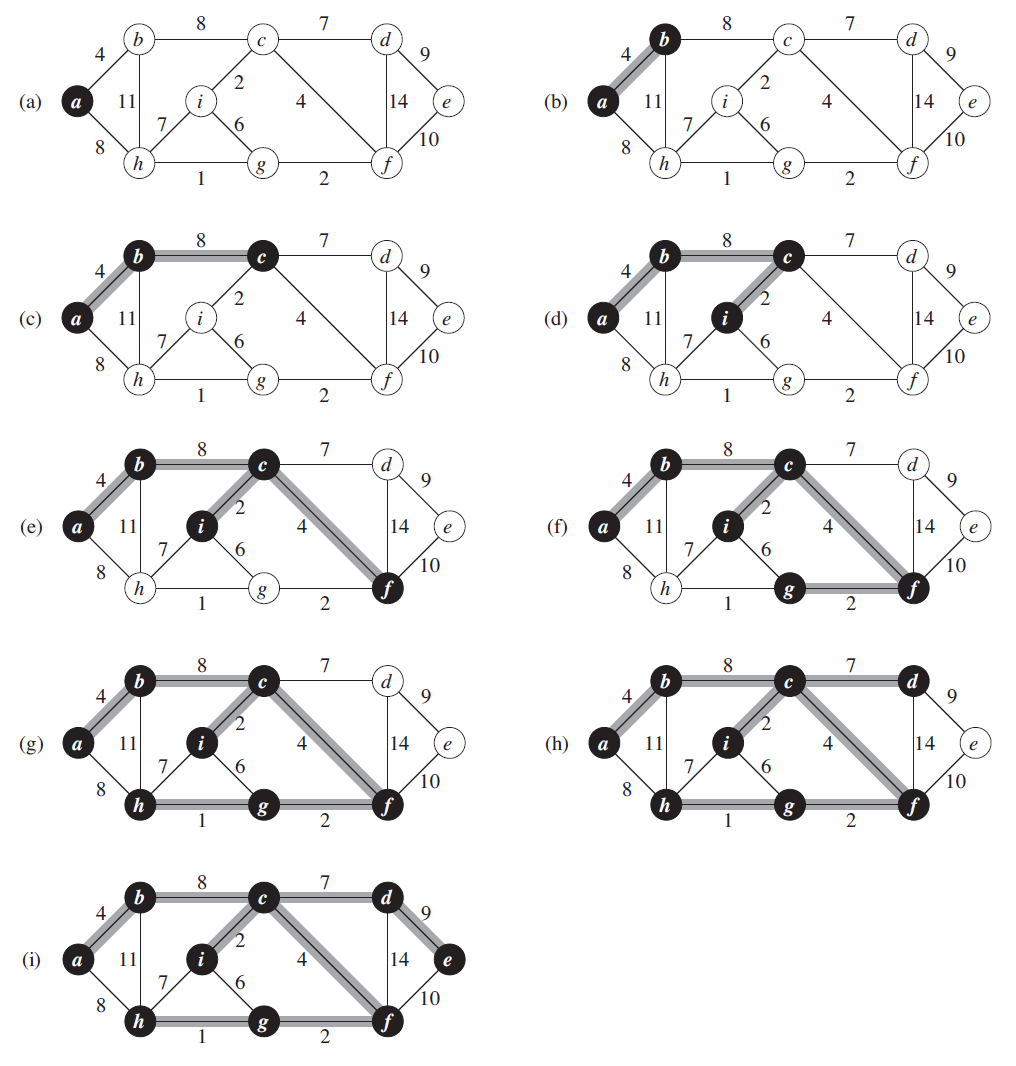
\includegraphics[width=\columnwidth]{prims-algorithm.png}
\end{figure}

\begin{enumerate}[(a)]
  \item 임의의 정점 $v_a$을 선택하고 집합 $T$에 추가한다. $D = (e_b^4, e_h^8)$.
  \item $T^c \land min(D) = e_b$와 그에 이어진 정점 $v_b$가 $T$에 없다면 추가한다. $D = (e_b^4, e_h^8, e_c^8)$. $v_b$와 이어진 $e_h^{11}$은 $D$에 있는 $e_h^8$보다 크므로 갱신하지 않음.
  \item $T^c \land min(D) = e_c$와 그에 이어진 정점 $v_c$가 $T$에 없다면 추가한다. $D = (e_b^4, e_h^8, e_c^8, e_i^2, e_f^4, e_d^7)$.
  \item 이렇게 정점과 간선을 하나씩 추가하다가 $T$에 추가된 간선의 개수가 $n - 1$개가 되면 종료한다.
\end{enumerate}

항상 $T$에 속하지 않은 정점을 추가하기 때문에 사이클이 만들어지지 않는다. 시간복잡도는 $O(n^2)$. 여기서 $n$은 정점 개수, 앞서 본 kruskal algorithm은 간선 개수이므로 일률적으로 비교가 불가하다.

\subsection{Dijkstra's Algorithm}

출발점에서 다른 모든 정점까지의 최단 경로를 찾는 알고리즘. 현재 정점에서 가중치가 가장 낮은 간선을 선택하고, 출발점에서 해당 간선에 이어진 정점까지의 가중치 총합을 기록해 다른 간선의 비용과 비교한다. 정점 s에서 출발해 다른 정점까지의 최단 거리를 구한다.

\begin{figure}[h]
  \centering
  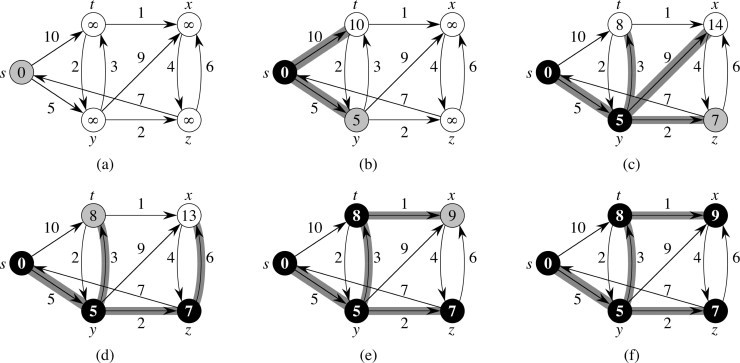
\includegraphics[width=\columnwidth]{dijkstra-algorithm.jpg}
\end{figure}

\begin{enumerate}[(a)]
  \item $s$에서 출발. 다른 정점까지의 거리를 모르기 때문에 모두 무한대.
  \item $s$와 이어진 $t=10, y=5$ 중 더 가까운 $y$ 선택.
  \item $t=8$로 갱신. $y$와 이어진 $t=8, x=14, z=7$ 중 가장 가까운 $z$ 선택.
  \item $x=13$으로 갱신. $y$와 이어진 $t=8, z$와 이어진 정점 $x=13$ 중 더 가까운 $t$ 선택.
  \item $x=9$로 갱신. $t$와 이어진 $x=9, x$ 선택.
  \item $s$로부터 모든 정점까지의 최단 거리를 알게 됨.
\end{enumerate}

시작점을 제외한 모든 정점에 대해 루프가 $(n - 1)$회 반복되고, 루프 내에서 최소의 점을 찾는 데 $O(n)$, 정점에 연결된 정점의 수가 최대 $O(n - 1)$개이므로 각 정점을 갱신하는 데 $O(n)$, 따라서 시간복잡도는 $(n - 1) \times \{O(n) + O(n)\} = O(n^2)$.

\subsection{Fractional Knapsack Problem}

배낭 문제는 결국 모든 경우의 수를 살펴야 하기 때문에 trivial하지 않은 문제. 하지만 부분 배낭 문제는 그리디 알고리즘으로 해결이 가능하다.

\begin{enumerate}[(a)]
  \item 각 물건의 단위 무게 당 가치를 계산한다: $O(n)$
  \item 가치를 기준으로 내림차순 정렬한다: $O(n \log{n})$
  \item 순서대로 담는다. 공간이 부족하면 최대 용량에서 현재 용량을 뺀 만큼만 담는다: $O(n)$
\end{enumerate}

\subsection{Set Cover Problem}

주어진 집합 $U$의 원소를 가장 많이 포함한 집합 $S$를 선택하는 과정을 반복. $S$를 선택하면 $U$에서 $S$에 포함되는 원소를 지운다. 이때 $S$를 찾으려면 남은 $S_i$들을 각각 $U$와 비교해야하므로 $O(n^2)$, 이를 $n$회 반복하므로 시간복잡도는 $O(n^3)$.

\subsection{Job Scheduling Problem}

작업 수행 시간이 중복되지 않도록 최소한의 머신에 배정하는 문제. 최적해를 찾으려면 빠른 시작 시간 작업 우선(earliest start time first) 배정해야 한다.

시작 시간이 빠른 순으로 작업 목록을 정렬하고($O(n \log{n})$, 가장 일찍 시작하는 작업부터 배정한다. 만약 시간이 겹친다면 새로운 머신을 만들어 배정한다($O(m)$, $m = \text{머신 수}$). 총 $n$번 루프를 실행하므로 시간복잡도는 $O(n \log{n}) + O(mn)$.

\subsection{Huffman Coding}

문자의 빈도수에 따라 이진 코드를 할당하고, 트리를 구성해 인코딩하는 알고리즘. 큐에서는 항상 빈도가 가장 낮은 정점 2개를 선택하며, 큐에 정점이 2개 미만이 되면 종료한다.

\begin{figure}[h]
  \centering
  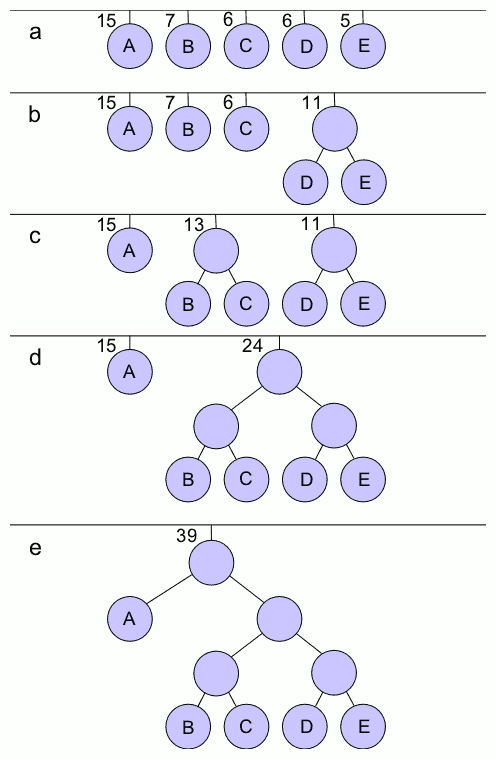
\includegraphics[width=\columnwidth]{huffman-coding-tree.png}
\end{figure}

\begin{enumerate}[(a)]
  \item 각 문자의 빈도수로 우선순위 큐를 만든다.
  \item 빈도수가 가장 작은 D(6), E(5) 정점을 \texttt{pop}해 새 정점 DE(11)의 하위 정점으로 만든다.
  \item 빈도수가 가장 작은 B(7), C(6) 정점을 \texttt{pop}해 새 정점 BC(13)의 하위 정점으로 만든다.
  \item 빈도수가 가장 작은 BC(13), DE(11) 정점을 \texttt{pop}해 새 정점 BCDE(24)의 하위 정점으로 만든다.
  \item 빈도수가 가장 작은 BCDE(24), A(15) 정점을 \texttt{pop}해 새 정점 BCDEA(39)의 하위 정점으로 만든다.
\end{enumerate}

\begin{figure}[h]
  \centering
  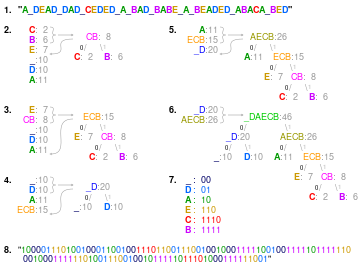
\includegraphics[width=\columnwidth]{huffman-coding-visual.png}
\end{figure}

여기서 왼쪽 간선에는 0, 오른쪽 간선에는 1을 부여하면 인코딩이 된다. 시간복잡도는 $O(n \log{n})$.

\section{Dynamic Programming}

최적화 문제를 해결하는 알고리즘. 문제를 쪼개서 해결한다는 점에서 분할 정복과 똑같지만, 다른 문제의 부분 문제를 사용한다는 점에서 다름. 가령 피보나치 수열을 분할 정복으로 구현하면 같은 문제를 중복해서 풀기 때문에 시간복잡도가 $O(2^n)$.

\begin{verbatim}
def f(n: int) -> int
  if n <= 1: return n
  return f(n - 1) + f(n - 2)
\end{verbatim}

동적 계획법으로 구현하면 효율적이다. 메모이제이션을 이용해 계산한 해를 테이블에 저장해두면 $O(n)$.

\begin{verbatim}
m = [0, 1] + [-1 for _ in range(n - 1)]
def f(n: int) -> int:
  if n <= 1:
    return n
  if m[n] == -1:
    m[n] = f(n - 1) + f(n - 2)
  return m[n]
\end{verbatim}

동적 계획법은 최적성 원칙 또는 최적 부분 구조라는 특성을 가지고 있음. 부분 문제들의 최적해를 이용해 원 문제에 대한 최적해를 구할 수 있다는 것. 즉, 문제의 최적해 속에 부분 문제의 최적해가 포함되어 있고, 부분 문제의 해 속에 그 보다 작은 부분 문제의 해가 포함되어 있다.

\subsection{Floyd-Warshall Algorithm}

모든 정점 쌍의 모든 최단 경로를 찾는 알고리즘. 다익스트라 알고리즘($O(n^2)$)을 $n$회 수행한 것과 같은 $O(n^3)$ 시간이 걸린다.

경로 표기 $D_{i,j}^k$는 정점 $1, 2, \cdots, k$의 경유를 고려한 정점 $i$부터 $j$까지의 모든 경로 중 가장 짧은 경로의 거리. ($k$를 경유할 수도, 경유하지 않을 수도 있다.) 따라서 $D_{i,j}^0$는 두 정점을 잇는 간선의 가중치를 의미한다.

\begin{figure}[h]
  \centering
  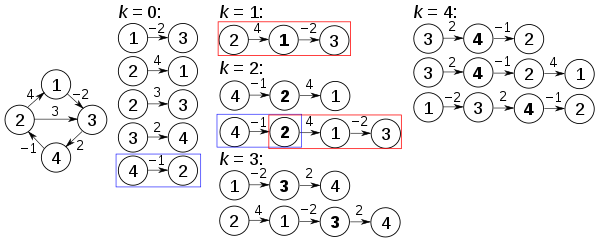
\includegraphics[width=\columnwidth]{floyd-warshall-algorithm.png}
\end{figure}

\begin{itemize}
  \item $k = 0$: 어떤 정점도 경유하지 않았을 때 도달할 수 있는 정점 목록.
  \item $k = 1$: 정점 1을 경유하는 최단 경로는 $D_{2,3}^1$ 하나. $D_{2,3}^0$보다 짧으므로 거리를 업데이트한다.
  \item $k = 2$: 정점 2를 경유하는 최단 경로의 목록. 이때 $D_{4,3}^2$는 $D_{4,2}^0$와 $D_{2,3}^1$의 합이다. 즉, $D_{i,j}^k = min(D_{i,j}^{k - 1}, D_{i,k}^{k - 1} + D_{k,j}^{k - 1})$. 다른 부분 문제의 해를 사용하는 동적 계획법의 예.
  \item $k = 3$: 정점 3을 경유하는 최단 경로의 목록.
  \item $k = 4$: 정점 4를 경유하는 최단 경로의 목록.
\end{itemize}

마지막 단계에서 모든 정점 간의 최단 거리를 알게 된다. 표로 표현하면 아래와 같다. 업데이트된 거리는 볼드체로 표기.

\begin{figure}[h]
  \centering
  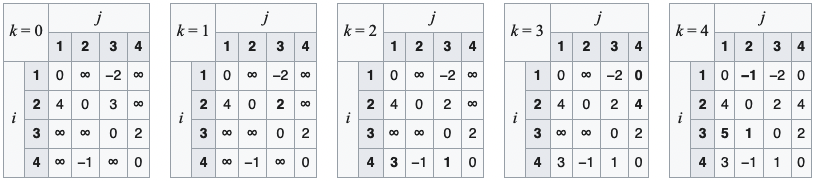
\includegraphics[width=\columnwidth]{floyd-warshall-table.png}
\end{figure}

\subsection{Matrix Chain Multiplication}

연속적인 행렬 곱을 효율적으로 계산하기 위한 연산 순서를 찾는 알고리즘. 행렬의 결합법칙을 이용.

\begin{verbatim}
def matrix_chain_mult(p: list[int],
                      n: int) -> int:
  m = [[0 for x in range(n)]
        for x in range(n)]

  for i in range(1, n):
    m[i][i] = 0

  for L in range(2, n):
    for i in range(1, n-L + 1):
      j = i + L-1
      m[i][j] = sys.maxsize
      for k in range(i, j):
        q = m[i][k] + m[k + 1][j]
            + p[i-1]*p[k]*p[j]
        if q < m[i][j]:
          m[i][j] = q

  return m[1][n-1]
\end{verbatim}

\subsection{Minimum Edit Distance}

두 문자열의 유사도를 판단하는 알고리즘. 어떤 문자열을 최소한의 횟수로 \texttt{insert}, \texttt{replace}, \texttt{delete}하여 다른 문자열로 변형. 모든 부분 문제에 대해 최소 동작 테이블을 만든다. 이때 $\rightarrow$: \texttt{insert}, $\searrow$: \texttt{replace}, $\downarrow$: \texttt{delete}.

\begin{figure}[h]
  \centering
  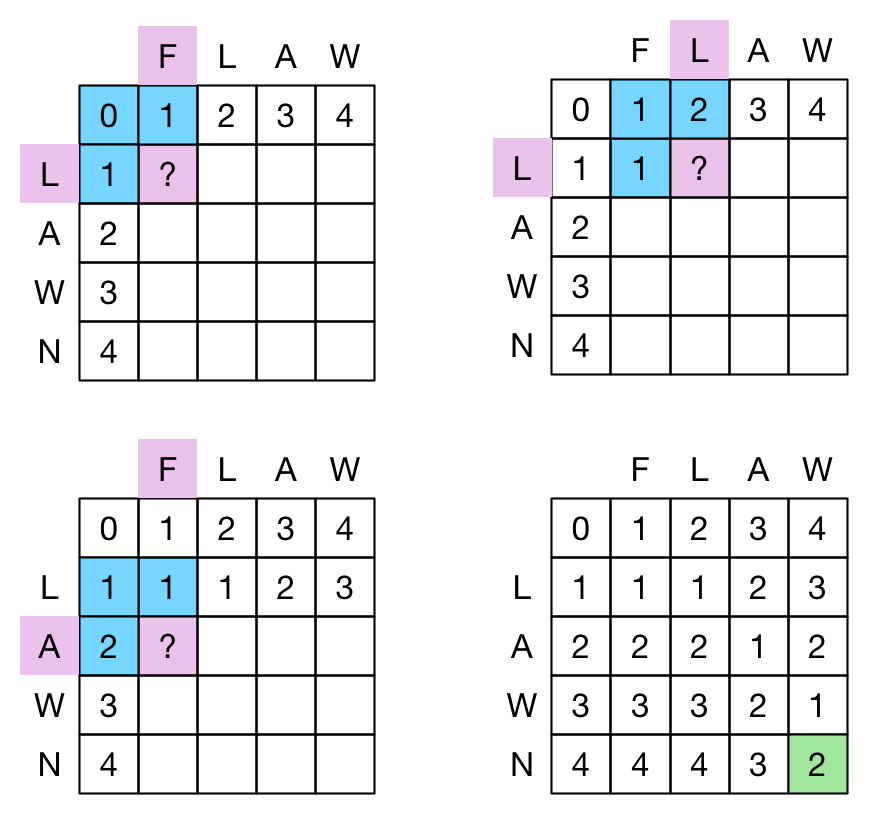
\includegraphics[width=\columnwidth]{minimum-edit-distance-table.png}
\end{figure}

예를 들어 LAWN를 FLAW로 변형하는 경우 최종적으로 2번의 변경이 필요하다.

\begin{enumerate}[(a)]
  \item L $\rightarrow$ F: min((1 + 1), (0 + 1), (1 + 1)) = 1.
  \item L $\rightarrow$ FL: min((1 + 1), (1 + 0), (2 + 1)) = 1.
  \item LA $\rightarrow$ F: min((2 + 1), (1 + 1), (1 + 1)) = 2.
  \item LAWN $\rightarrow$ FLAW: min((3 + 1), (2 + 1), (1 + 1)) = 2.
\end{enumerate}

\begin{verbatim}
def minimum_edit_distance(x: str,
                          y: str) -> int:
  (m, n) = (len(x), len(y))

  t = [[0 for _ in range(n + 1)]
        for _ in range(m + 1)]

  for i in range(m + 1): t[i][0] = i
  for j in range(n + 1): t[0][j] = j

  c = 0
  for i in range(1, m + 1):
    for j in range(1, n + 1):
      if x[i - 1] == y[j - 1]:
        c = 0
      else:
        c = 1
      t[i][j] = min(t[i][j - 1] + 1,
                    t[i - 1][j - 1] + c,
                    t[i - 1][j] + 1)

  return t[m][n]
\end{verbatim}

시간복잡도는 테이블을 만드는 시간: $O(mn)$.

\subsection{1-0 Knapsack Problem}

$n$개의 물건과 각 물건의 무게 $w_i$와 가치 $v_i$가 주어지고, 배낭의 용량이 $c$일 때, 배낭에 담을 수 있는 물건의 최대 가치를 찾는 문제. 각 물건이 배낭에 담기지 않는 경우는 0, 담긴 경우는 1로 취급.

\begin{verbatim}
def knapsack(s: list[tuple[int, int]],
             c: int) -> int:
  sl = len(s)
  t = [[0 for _ in range(c)]
        for _ in range(sl - 1)]

  for i in range(1, sl):
    for w in range(1, c):
      wi = s[0][i]
      vi = s[1][i]
      if (wi > w):
        t[i, w] = t[i - 1, w]
      else:
        t[i, w] = max(t[i - 1, w],
                      t[i - 1, w - wi] + si)
  return t[n, c]
\end{verbatim}

배낭 문제는 NP-Complete 문제. P 문제는 다항 시간 내에 해결할 수 있는 문제, NP 문제는 다항 시간 내에 해결할 수 없는 문제. NP-Hard 문제는 NP에 속하는 어떤 문제를 다항 시간 내에 다른 문제로 변경할 수 있는 문제. NP-Complete 문제는 NP이면서 NP-Hard인 문제.

\subsection{Coin Change Problem}

동전 거스름돈 문제를 그리디하게 해결하려면 적절한 동전 단위가 전제되어야 한다. 다양한 단위의 거스름돈을 다루기 위해 $0$부터 $n$원까지의 테이블을 만든다. 동전의 단위가 $d_{16} = 16$, $d_{10} = 10$, $d_5 = 5$, $d_1 = 1$원일 때 20원을 거슬러줘야 한다면.

\begin{enumerate}[(a)]
  \item $0$부터 $20$까지의 배열 $C$를 $C[0] = 0$, 그 외는 무한대로 초기화.
  \item $C[i_1]$: $d_1 \leq i_1$, $C[i_1 - d_1] + 1 = 1$.
  \item $C[i_2]$: $d_1 \leq i_2$, $C[i_2 - d_1] + 1 = 2$.
  \item $C[i_5]$: $d_5 \leq i_5$, $C[i_5 - d_5] + 1 = 1$. $d_1 \geq i_5$ 조건도 참이긴 하지만, $C[i_5 - d_1] + 1 < C[i_5] = C[4] + 1 < C[i_5] = 4 < 1$ 조건을 만족하지 않음.
  \item $C[i_{20}]$: $d_{16} \leq i_{20}$, $C[i_{20} - d_{16}] + 1 = 5$. 그런데 $C[i_{20} - d_{10}] + 1 < C[i_{20}] = C[10] + 1 < 5 = 2 < 5$ 조건을 만족하므로 $2$로 갱신.
\end{enumerate}
